\documentclass{beamer}

\usepackage{graphicx}
\usepackage{amsmath}
\usepackage{framed}

\begin{document}
	
	% = http://cran.rstudio.com/web/packages/dplyr/vignettes/introduction.html
\begin{frame}
	\begin{figure}
		\centering
		
\includegraphics[width=0.78\linewidth]{images/dplyr-title}
	\end{figure}
\end{frame}
%===============================================%
\begin{frame}
\begin{figure}
\centering
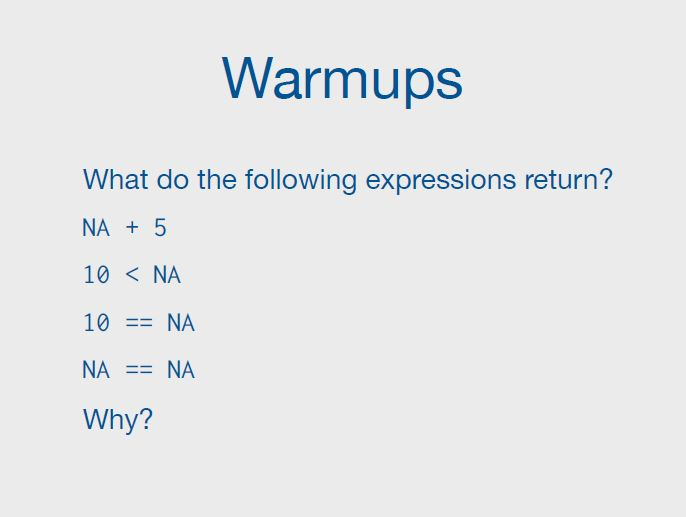
\includegraphics[width=1.05\linewidth]{images/CG-dplyr1}
\end{figure}
\end{frame}
%===============================================%
\begin{frame}
	\begin{figure}
		\centering
		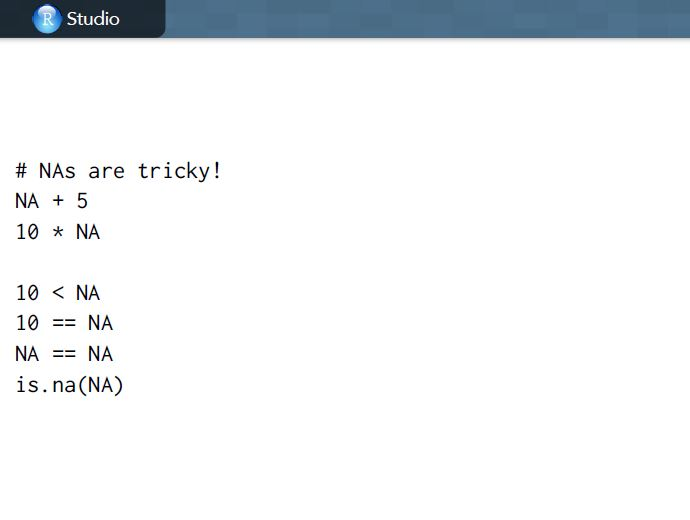
\includegraphics[width=1.05\linewidth]{images/CG-dplyr2}
	\end{figure}
\end{frame}
%===============================================%
\begin{frame}
	\begin{figure}
		\centering
		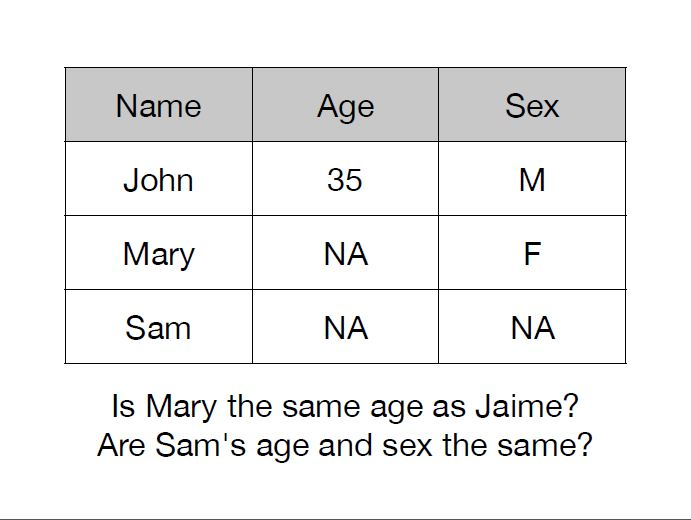
\includegraphics[width=1.05\linewidth]{images/CG-dplyr3}
	\end{figure}
\end{frame}
%===============================================%
\begin{frame}
	\begin{figure}
		\centering
		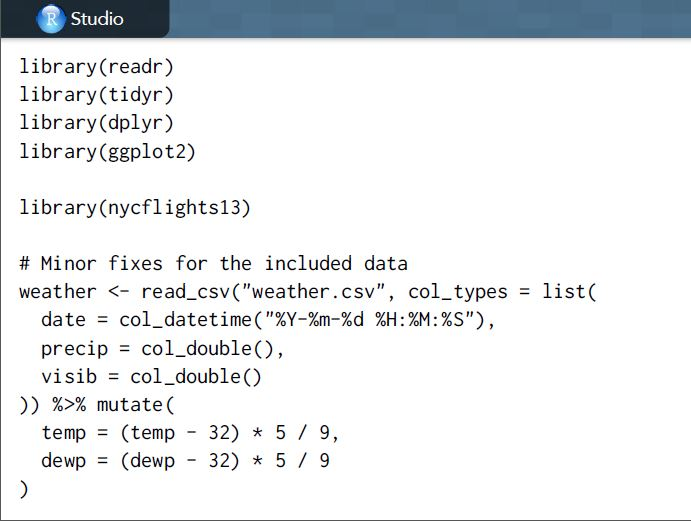
\includegraphics[width=1.05\linewidth]{images/CG-dplyr4}
	\end{figure}
\end{frame}
%===============================================%
\begin{frame}
	\begin{figure}
		\centering
		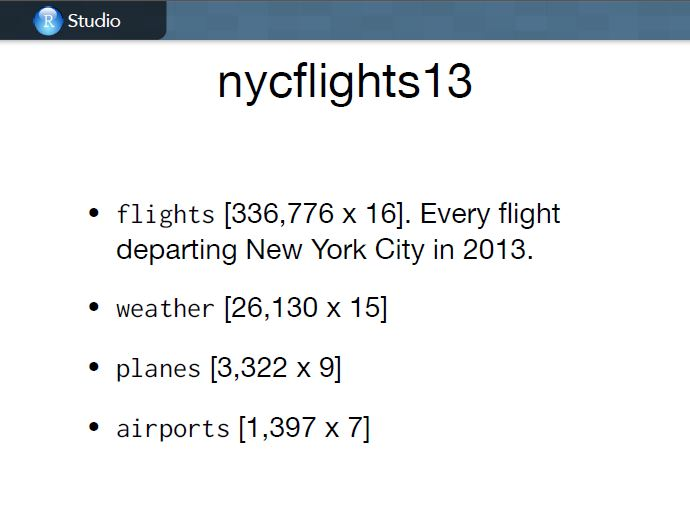
\includegraphics[width=1.05\linewidth]{images/CG-dplyr5}
	\end{figure}
\end{frame}
%===============================================%
\begin{frame}
	\begin{figure}
		\centering
		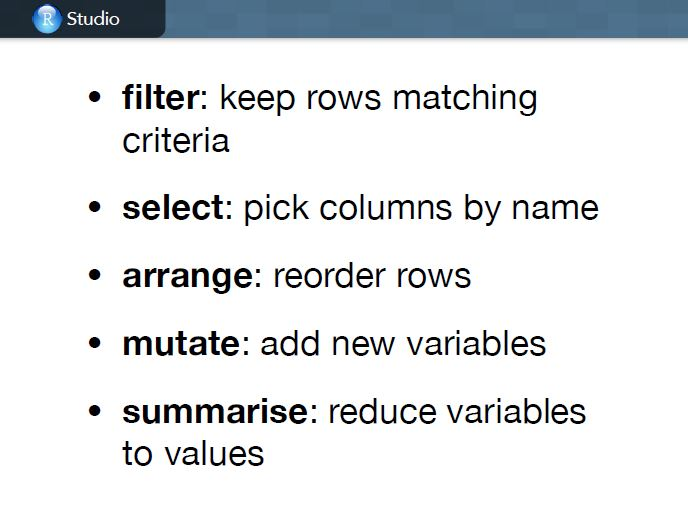
\includegraphics[width=1.05\linewidth]{images/CG-dplyr6}
	\end{figure}
\end{frame}
%===============================================%
\begin{frame}
	\begin{figure}
		\centering
		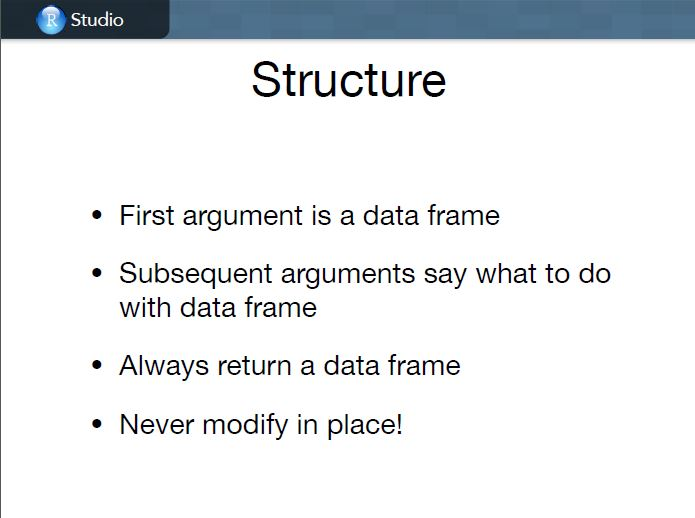
\includegraphics[width=1.05\linewidth]{images/CG-dplyr7}
	\end{figure}
\end{frame}
%===============================================%
\begin{frame}
	\begin{figure}
		\centering
		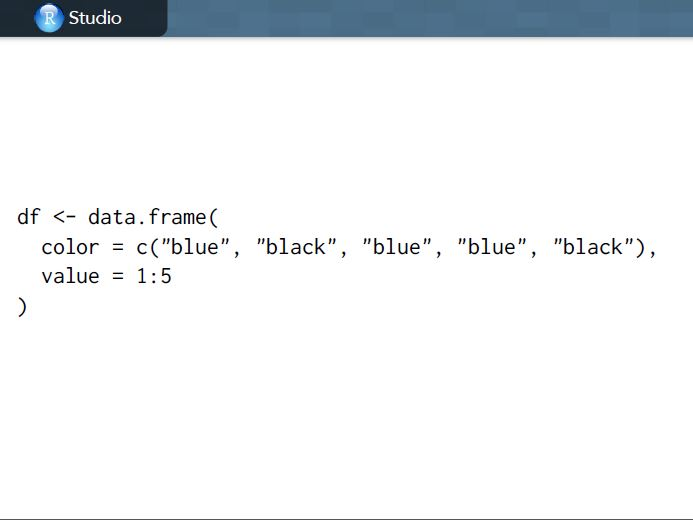
\includegraphics[width=1.05\linewidth]{images/CG-dplyr8}
	\end{figure}
\end{frame}
%===============================================%
\begin{frame}
	\begin{figure}
		\centering
		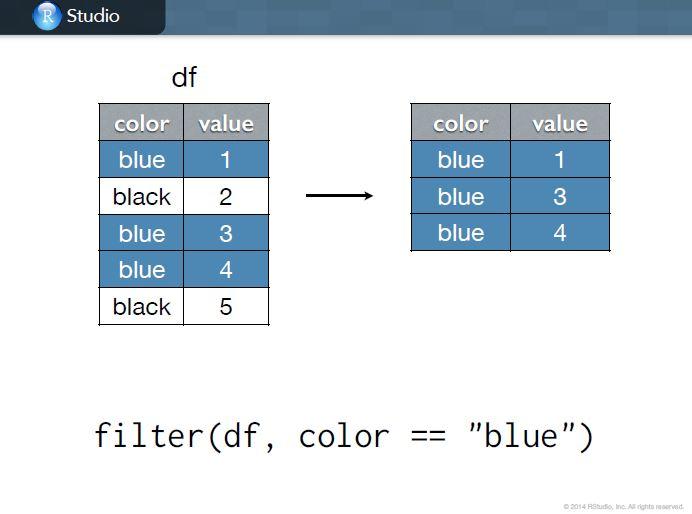
\includegraphics[width=1.05\linewidth]{images/CG-dplyr9}
	\end{figure}
\end{frame}
%===============================================%
\begin{frame}
	\begin{figure}
		\centering
		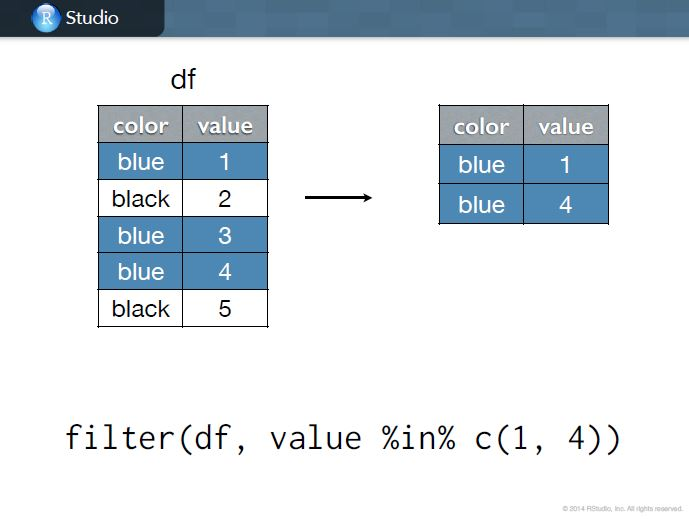
\includegraphics[width=1.05\linewidth]{images/CG-dplyr10}
	\end{figure}
\end{frame}
\begin{frame}
	\begin{figure}
		\centering
		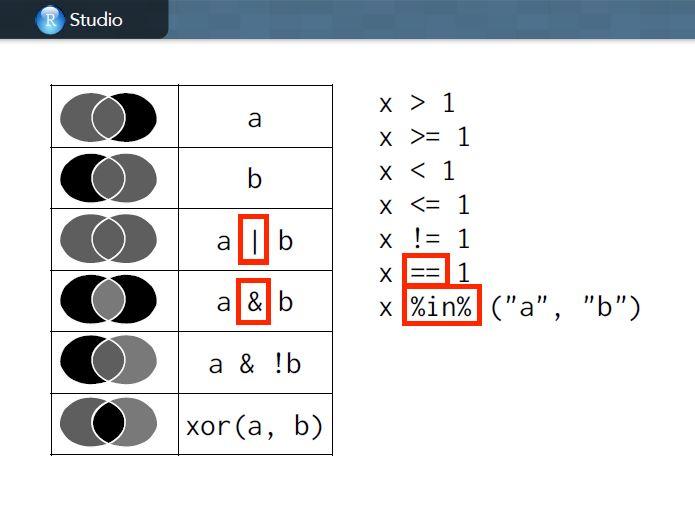
\includegraphics[width=1.05\linewidth]{images/CG-dplyr11}
	\end{figure}
\end{frame}
%===============================================%
\begin{frame}
	\begin{figure}
		\centering
		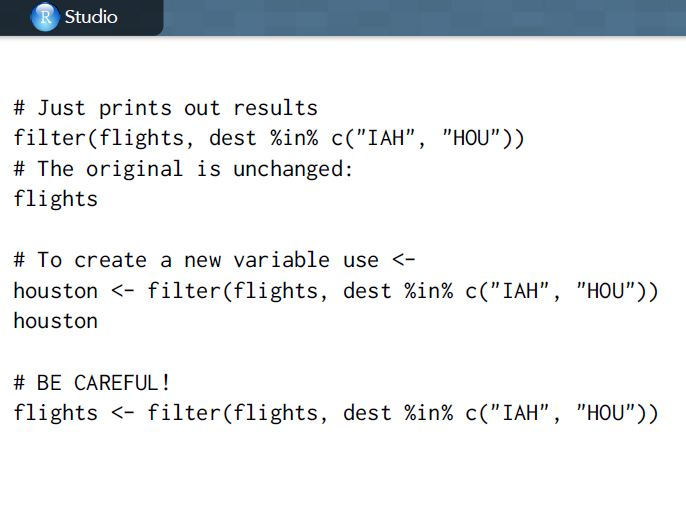
\includegraphics[width=1.05\linewidth]{images/CG-dplyr12}
	\end{figure}
\end{frame}


\end{document}